\documentclass[aspectratio=169,xcolor=table,10pt, notes=hide]{beamer}


\usetheme[faculty=phil]{fibeamer}
\usepackage{polyglossia}

\setmainlanguage{russian} %% main locale instead of `english`, you
%% can typeset the presentation in either Czech or Slovak,
%% respectively.
\setotherlanguages{english} %% The additional keys allow
%%
%%   \begin{otherlanguage}{czech}   ... \end{otherlanguage}
%%   \begin{otherlanguage}{slovak}  ... \end{otherlanguage}
%%
%% These macros specify information about the presentation
\title[Theoretical Mechanics]{Theoretical Mechanics, Lab 2: KIN ROT PLANE1} %% that will be typeset on the
\subtitle{Rotational Motion \\ Plane Motion: Intro \\ \  } %% title page.
\author{Oleg Bulichev}
%% These additional packages are used within the document:
\usepackage{ragged2e}  % `\justifying` text
\usepackage{booktabs}  % Tables
\usepackage{tabularx}
\usepackage{tikz}      % Diagrams
\usetikzlibrary{decorations.pathreplacing,calligraphy,calc,graphs, shapes, backgrounds}
\usepackage{amsmath, amssymb}
\usepackage{url}       % `\url`s
\usepackage{listings}  % Code listings
\usepackage{floatrow}
\usepackage{mathtools}
\usepackage{fontspec}
\usepackage{multicol}
\usepackage{pdfpages}
\usepackage{wrapfig}
\usepackage{animate}
\usepackage{booktabs}
\usepackage{multirow}
\usepackage{multimedia}
\usepackage{makecell}
\usepackage{colortbl}
\usepackage{hhline}
\usepackage{rotating}
\usepackage{amsmath}

\usepackage[font={}, labelfont=it,textfont={it},justification=centering, skip=0pt]{caption}
% will apply to all subcaptions
\usepackage[font={},skip=2pt]{subcaption}


\graphicspath{{resources/}}
\frenchspacing




% \setbeamertemplate{caption}[numbered]
\captionsetup[figure]{labelformat=empty}


\newcommand{\fbckg}[1]{\usebackgroundtemplate{\includegraphics[width=\paperwidth]{#1}}}%frame background

\usepackage[framemethod=TikZ]{mdframed}
\newcommand{\dbox}[1]{
\begin{mdframed}[roundcorner=3pt, backgroundcolor=yellow, linewidth=0]
\vspace{1mm}
{#1}
\vspace{1mm}
\end{mdframed}
}
\addtobeamertemplate{frametitle}{}{\vspace{-0.35cm}}

% \usepackage{pgfpages}
% \pgfpagesuselayout{4 on 1}[a4paper,border shrink=2mm,landscape]
\usepackage{color}
\usepackage{rotating}
\usepackage{tabularray}

\begin{document}
\setlength{\abovedisplayskip}{0pt}
\setlength{\belowdisplayskip}{0pt}
\setlength{\abovedisplayshortskip}{0pt}
\setlength{\belowdisplayshortskip}{0pt}

\fbckg{fibeamer/figs/title_page.png}
\frame[c]{\setcounter{framenumber}{0}
    \usebeamerfont{title}%
    \usebeamercolor[fg]{title}%
    \begin{minipage}[b][6.3\baselineskip][b]{\textwidth}%
        \textcolor{black}{\raggedright\inserttitle}
    \end{minipage}
    % \vskip-1.5\baselineskip

    \usebeamerfont{subtitle}%
    \usebeamercolor[fg]{framesubtitle}%
    \begin{minipage}[b][3\baselineskip][b]{\textwidth}
        \raggedright%
        \insertsubtitle%
    \end{minipage}
    \vskip.25\baselineskip
}

\note{}

\fbckg{fibeamer/figs/common.png}

\section*{Motion representation}

\begin{frame}[t]{Formulas}
    \footnotesize
    $y = y(x)$ -- trajectory in geometry space (can be called as equation of the path)

    \centering\textbf{Forms}
    \vspace{-0.3cm}
    \begin{multicols}{3}
        \begin{enumerate}
            \footnotesize
            \item Radius vector $\vec{r} = \vec{r}(t)$
            \item Coordinate $\begin{matrix} x = x(t)\\y = y(t)\\z = z(t)\end{matrix}$
            \item Natural (arc length) $\sigma = \sigma(t)$
        \end{enumerate}
    \end{multicols}
    \vspace{-0.3cm}
    \begin{columns}[T,onlytextwidth]
        \begin{column}{0.42\textwidth}
            % \vspace{1 cm}
            \textbf{Transformations (general)}
            \begin{itemize}
                \footnotesize
                \item $2 \rightarrow 1$; $\vec{r} = \begin{bmatrix}x(t)\\y(t)\\z(t)\end{bmatrix} = x\vec{i} + y\vec{j} + z\vec{k}$
                \item $1 \rightarrow 2$; $\begin{matrix} x\\ y\\ z \end{matrix} = \begin{bmatrix}
                              \cos(\alpha_{rx})\vec{r} \\
                              \cos(\alpha_{ry})\vec{r} \\
                              \cos(\alpha_{rz})\vec{r}
                          \end{bmatrix}$
                \item $2 \rightarrow 3$; $\sigma(t)=\int \limits _{0}^{t}{\sqrt {\dot{x}^2 + \dot{y}^2 + \dot{z}^2}}dt$ -- useless without knowing trajectory. Also, you are losing signs. \href{https://youtu.be/Hfn0Oj\_METo?si=omTZDwwpof7N9uwd}{More Info}.
            \end{itemize}

        \end{column}
        \begin{column}{0.60\textwidth}
            \textbf{Transformations (planar)}
            \vspace{-0.3cm}
            \begin{multicols}{2}
                \begin{itemize}
                    \footnotesize
                    \item $2 \rightarrow 1$; $\vec{r} = \begin{bmatrix}x(t)\\y(t)\\\end{bmatrix} = x\vec{i} + y\vec{j}$
                    \item $1 \rightarrow 2$; $\begin{matrix} x\\ y\end{matrix} = \begin{bmatrix}
                                  cos(\alpha_{rx})\vec{r} \\
                                  cos(\alpha_{ry})\vec{r} \\\end{bmatrix}$
                \end{itemize}
            \end{multicols}
            \vspace{-0.3cm}
            \begin{itemize}
                \footnotesize
                \item $2 \rightarrow 3$; $\sigma(t)=\int \limits _{0}^{t}{\sqrt {\dot{x}^2 + \dot{y}^2}}dt$ -- in practice, useless without knowing trajectory.
                \item $1(2) \rightarrow y(x) \rightarrow \sigma(x)$; $\sigma(x)=\int \limits _{a}^{b}{\sqrt {1+(y'(x))^{2}}}dx$ works if $y$ is unique for each $x$
                \item $\sigma(x) \rightarrow y(x) \rightarrow 1(2)$; $\sigma_{cur} - \sigma(x) =0$.\\ Can be solved, using numerical optimization or brute force. \href{https://en.wikipedia.org/wiki/Differentiable\_curve\#Length\_and\_natural\_parametrization}{Info}.
            \end{itemize}
        \end{column}
    \end{columns}
\end{frame}

\begin{frame}[t]{Linear and angular components of rigid body motion}
    \footnotesize
    \begin{columns}[T,onlytextwidth]
        \begin{column}{0.49\textwidth}
            \textbf{Linear part} \\
            Position type -- 1 = $\vec{r}$ \\
            Velocity type -- 1 = $\vec{V}$, Speed =  $|\vec{V}|$ \\
            $\vec{V} = \frac{\mathrm{d} \vec{r}}{\mathrm{d} t} = \dot{x}\vec{i} + \dot{y}\vec{j} + \dot{z}\vec{k} = \dot{\sigma}\vec{\tau} $ \\
            Velocity is always tangent to the trajectory function \\
            Path function is $f$ \\
            $y = f'(x)(x-x_{cur})+f(x_{cur})$ --- easy to convert to $\vec{\tau}$ \\
            Acceleration types -- 2: tangent and normal = $\vec{a}_{\tau},\ \vec{a}_{n}$ \\
            $\vec{a} = \ddot{x}\vec{i} + \ddot{y}\vec{j} + \ddot{z}\vec{k} = \vec{a}_{\tau} + \vec{a}_{n} $\\
            $\vec{a}_{\tau} = \ddot{\sigma} \vec{\tau} = \frac{\vec{a} \cdot \vec{V}}{V} \vec{\tau}$ \\
            $\vec{a}_{n} = \frac{\dot{\sigma}^2}{\rho}\vec{n} =\frac{|\vec{a} \times \vec{V}|}{V}\vec{n}$\\
            $\rho = \frac{1}{\kappa}$, where $\kappa$ is curvature \\
            $\kappa (x)=\frac {|f''|}{({\sqrt {1+f'^{2}}})^{3}}$
        \end{column}
        \begin{column}{0.49\textwidth}
            \textbf{Angular part} \\
            All of these guys are pseudovectors. We can put them wherever we want.\\
            Angle type -- 1 = $\vec{\phi}$\\
            Angular velocity type -- 1 = $\vec{\omega}$\\
            Angular acceleration -- 1 (on a plane) = $ \vec{\varepsilon}$

            \bigskip

            \textbf{Linear $\leftrightarrow$ Angular} \\
            $ \vec{v} = \vec{\omega} \times \vec{r}$ \\
            $ \vec{a}_{\tau} = \vec{\varepsilon} \times \vec{r}$ \\
            $ \vec{a}_{n} = \vec{\omega} \times (\vec{\omega} \times \vec{r})$
        \end{column}
    \end{columns}

\end{frame}

\section*{Rotational motion}

\begin{frame}[t]{Task 1 (yours)}
    \framesubtitle{}
    \begin{columns}[c,onlytextwidth]
        \begin{column}{0.55\textwidth}
            Point $M$ moves on a circle $R=60$. Motion law is given in natural form $s=\smallsmile OM = \frac{\pi R}{6}(3t-t^2) $. You should find velocity and acceleration, when t = 1.
            \medskip

            \textit{Answer}: $a_n = 16.4,\ a_\tau = -62.8,\ a = 64.9,\ v = 31.4$
        \end{column}
        \begin{column}{0.44\textwidth}
            \begin{figure}[H]
                \centering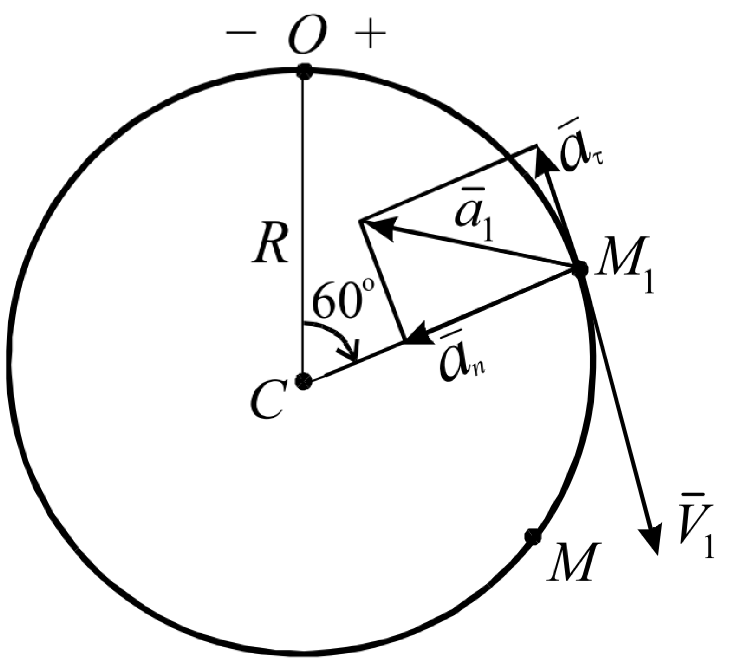
\includegraphics[height=5cm,width=1\textwidth,keepaspectratio]{image9.png}
                \caption*{Task 1}
                \label{fig:image9.png}
            \end{figure}
        \end{column}
    \end{columns}
\end{frame}

\begin{frame}[t]{Task 2 (mine)}
    \framesubtitle{}
    \begin{columns}[c,onlytextwidth]
        \begin{column}{0.59\textwidth}
            Disk $R = 2$ rotates around $O$. Its motion is $\phi = \phi(t) = 2e^{-2t}$. It is needed to find angular velocity and angular acceleration for the body. Also, you need to find $v_M,\ a_M$ for $t=0$.
        \end{column}
        \begin{column}{0.39\textwidth}
            \begin{figure}[H]
                \centering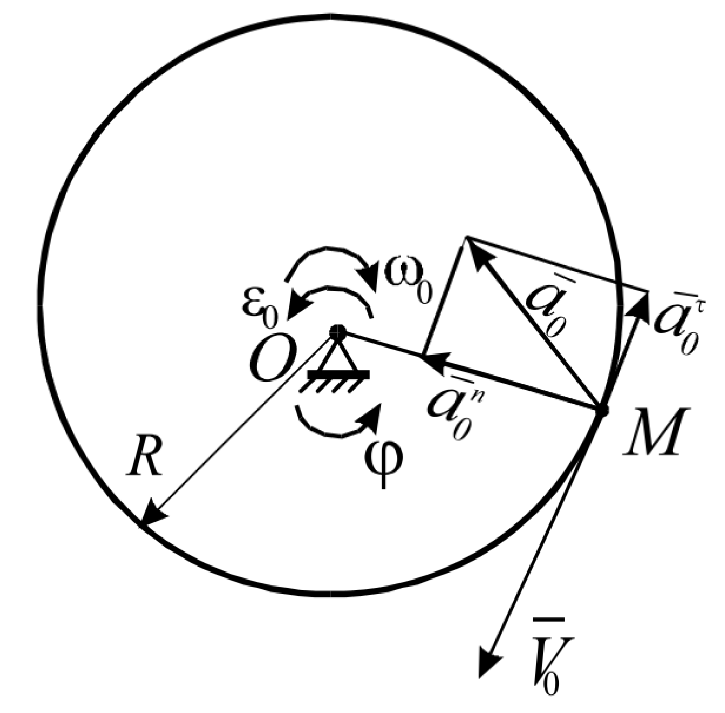
\includegraphics[height=5cm,width=1\textwidth,keepaspectratio]{image8.png}
                \caption*{Task 2}
                \label{fig:image8.png}
            \end{figure}
        \end{column}
    \end{columns}
\end{frame}

\begin{frame}[t]{Task 3 (mine)}
    \framesubtitle{}
    \begin{columns}[c,onlytextwidth]
        \begin{column}{0.59\textwidth}
            The mechanism contains 2 wheels: \textbf{1}, $R_1 = 4$, and \textbf{2}, $R_2=2,\ r_2 = 1$, which are connected with a toothed bar \textbf{3}. We also know the motion law of \textbf{1}, $\phi(t) = 4t-t^2$.
            \medskip
            Tasks:
            \begin{enumerate}
                \item For t = 1, find acceleration and velocity for \textbf{3}
                \item Find all types of acceleration for $A$.
            \end{enumerate}
        \end{column}
        \begin{column}{0.39\textwidth}
            \begin{figure}[H]
                \centering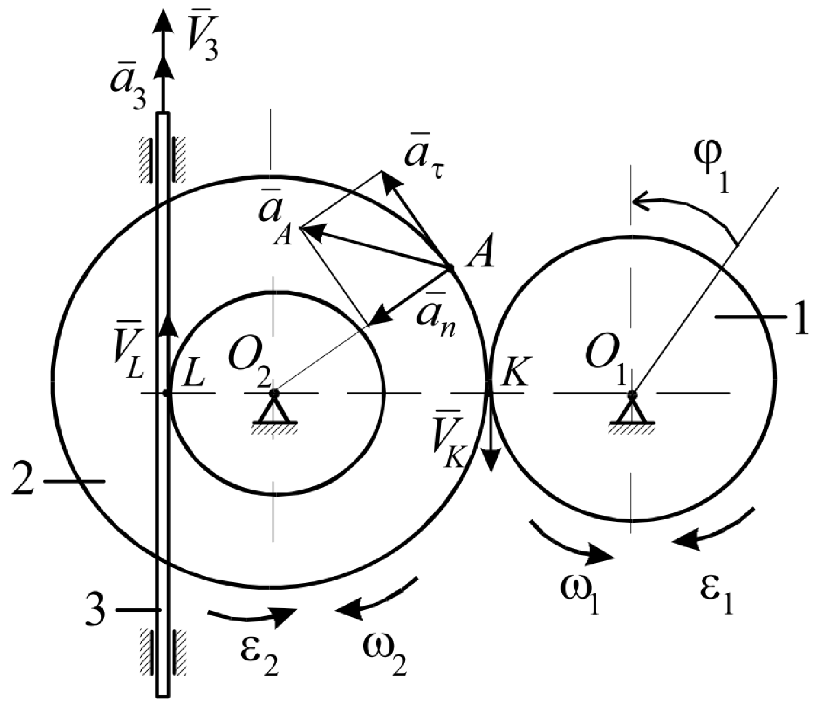
\includegraphics[height=6cm,width=1\textwidth,keepaspectratio]{image14.png}
                \caption*{Task 3}
                \label{fig:image14.png}
            \end{figure}
        \end{column}
    \end{columns}
\end{frame}

\section*{Plane motion}

\begin{frame}[t]{How to find velocities and acc of a rigid body}
    \framesubtitle{}
    \textbf{Velocity} \\
    \textit{Approaches}:
    1) Analytical 2) Instantaneous centre of zero velocity 3) Geometrically
    \medskip

    We need to think about direction, length.

    Notation: if know $\underline{1}, \underline{\underline{\text { both }}}$ \\
    $\vec{v}_b=\vec{v}_a+\vec{v}_{b a}=\vec{v}_a+\vec{\omega} \times \vec{r}_{b a}$\\
    \textbf{Accelerations} \\
    \textit{Approaches}: 1) Analytical \\
    $
        \vec{a}=\vec{a}_a+\vec{a}_{b a}^\tau+\vec{a}_{b a}^n=\vec{a}_a+\vec{\varepsilon} \times \vec{r}_{b a}+\vec{\omega} \times\left(\vec{\omega} \times \vec{r}_{b a}\right)
    $
\end{frame}


\begin{frame}[t]{Task 4 (mine)}
    \framesubtitle{}
    \begin{columns}[c,onlytextwidth]
        \begin{column}{0.59\textwidth}
            You should simulate this mechanism (obtain all positions) ($x_i(t),\ y_i(t)$, where $i$ are $A,\ B,\ C$ points)
            \medskip
            If $\omega_{OA} = const = 1$; $t$ --- 1 cycle \\
            $OA = 35,\ AB=70,\ AC=45$.
        \end{column}
        \begin{column}{0.39\textwidth}
            \begin{figure}[H]
                \centering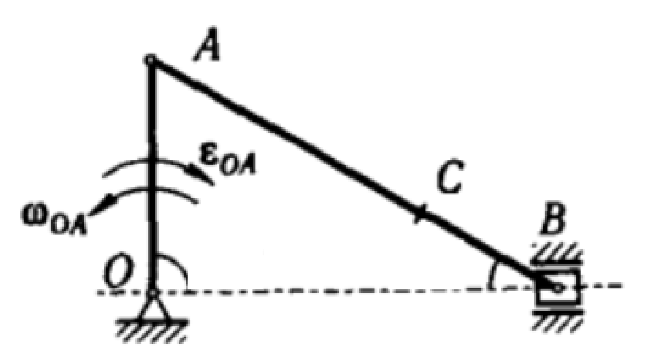
\includegraphics[height=5cm,width=1\textwidth,keepaspectratio]{image21.png}
                \caption*{Task 4}
                \label{fig:image21.png}
            \end{figure}
        \end{column}
    \end{columns}
\end{frame}

\begin{frame}[t]{Task 4 (mine)}
    \framesubtitle{Simulation in Geogebra}
    \begin{figure}[H]
        \href{https://www.geogebra.org/calculator/jukgsc8y}{
            \centering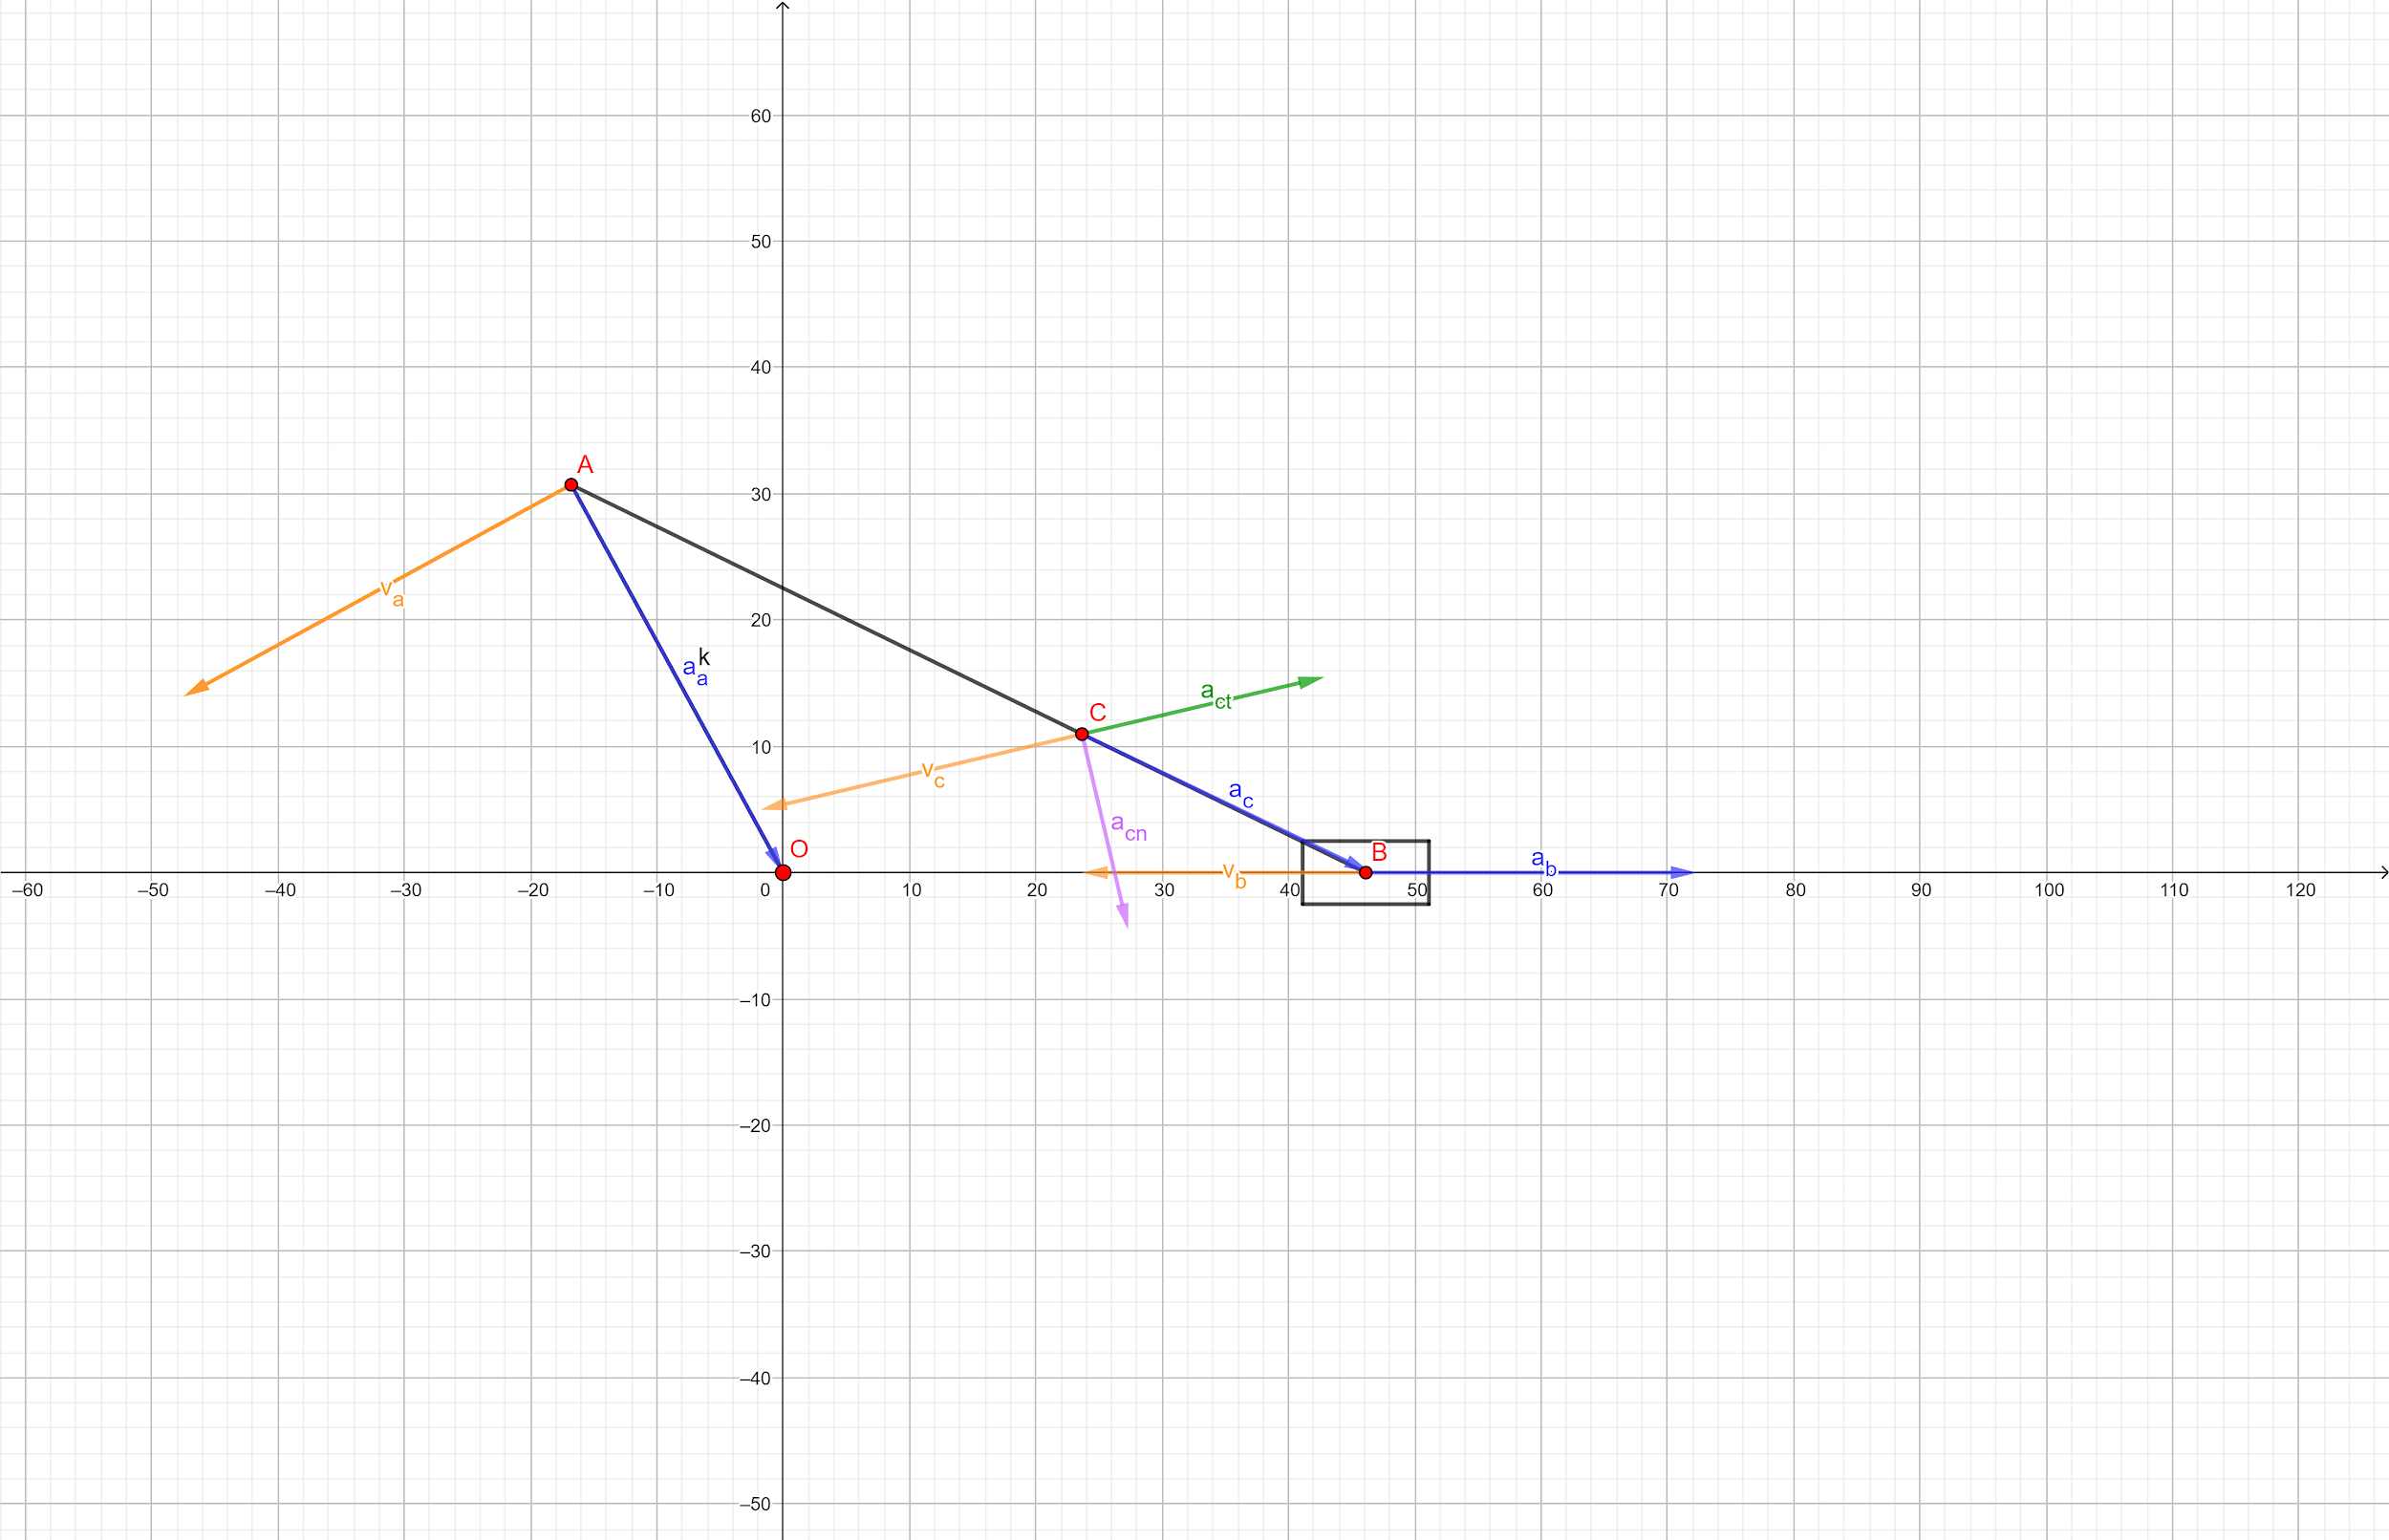
\includegraphics[height=6cm,width=1\textwidth,keepaspectratio]{image25.png}}
        \label{fig:image25.png}
    \end{figure}
\end{frame}

\begin{frame}[t]{3 typical approaches for kinematics}
    \begin{columns}[T,onlytextwidth]
        \begin{column}{0.32\textwidth}
            \textbf{Triangular}

            Consider a mechanics as a set of triangles.

            \textbf{Solution based on}

            Sin and Cosine rules mainly.

            +: fast, easy to code.

            -: applicable only for simple mechanisms
        \end{column}
        \begin{column}{0.32\textwidth}
            \textbf{Geometrical}

            Represent a mechanism as a set
            of figures (mainly circles and lines)

            \textbf{Solution based on}

            Finding intersection b/w figures (line-line,circle-line,circle-circle,sphere-line). Need nonlinear
            solver!

            +: Solve most of mech.,
            choosing roots are intuitive

            -: difficult to imagine
        \end{column}
        \begin{column}{0.32\textwidth}
            \textbf{Vector-based}

            Represent a mechanism
            as a set of vectors

            \textbf{Solution based on}

            Writing a system of
            nonlinear equations and
            put it in nonlinear solver!

            +: Best for tough mech.,
            easy to imagine

            -: Need to prepare a
            solver for finding roots
        \end{column}
    \end{columns}
\end{frame}

\fbckg{fibeamer/figs/last_page.png}
\frame[plain]{}
\fbckg{fibeamer/figs/common.png}

\end{document}

